\documentclass[handout]{ximera}

%% You can put user macros here
%% However, you cannot make new environments



\newcommand{\ffrac}[2]{\frac{\text{\footnotesize $#1$}}{\text{\footnotesize $#2$}}}
\newcommand{\vasymptote}[2][]{
    \draw [densely dashed,#1] ({rel axis cs:0,0} -| {axis cs:#2,0}) -- ({rel axis cs:0,1} -| {axis cs:#2,0});
}


\graphicspath{{./}{firstExample/}}
\usepackage{forest}
\usepackage{amsmath}
\usepackage{amssymb}
\usepackage{array}
\usepackage[makeroom]{cancel} %% for strike outs
\usepackage{pgffor} %% required for integral for loops
\usepackage{tikz}
\usepackage{tikz-cd}
\usepackage{tkz-euclide}
\usetikzlibrary{shapes.multipart}


%\usetkzobj{all}
\tikzstyle geometryDiagrams=[ultra thick,color=blue!50!black]


\usetikzlibrary{arrows}
\tikzset{>=stealth,commutative diagrams/.cd,
  arrow style=tikz,diagrams={>=stealth}} %% cool arrow head
\tikzset{shorten <>/.style={ shorten >=#1, shorten <=#1 } } %% allows shorter vectors

\usetikzlibrary{backgrounds} %% for boxes around graphs
\usetikzlibrary{shapes,positioning}  %% Clouds and stars
\usetikzlibrary{matrix} %% for matrix
\usepgfplotslibrary{polar} %% for polar plots
\usepgfplotslibrary{fillbetween} %% to shade area between curves in TikZ



%\usepackage[width=4.375in, height=7.0in, top=1.0in, papersize={5.5in,8.5in}]{geometry}
%\usepackage[pdftex]{graphicx}
%\usepackage{tipa}
%\usepackage{txfonts}
%\usepackage{textcomp}
%\usepackage{amsthm}
%\usepackage{xy}
%\usepackage{fancyhdr}
%\usepackage{xcolor}
%\usepackage{mathtools} %% for pretty underbrace % Breaks Ximera
%\usepackage{multicol}



\newcommand{\RR}{\mathbb R}
\newcommand{\R}{\mathbb R}
\newcommand{\C}{\mathbb C}
\newcommand{\N}{\mathbb N}
\newcommand{\Z}{\mathbb Z}
\newcommand{\dis}{\displaystyle}
%\renewcommand{\d}{\,d\!}
\renewcommand{\d}{\mathop{}\!d}
\newcommand{\dd}[2][]{\frac{\d #1}{\d #2}}
\newcommand{\pp}[2][]{\frac{\partial #1}{\partial #2}}
\renewcommand{\l}{\ell}
\newcommand{\ddx}{\frac{d}{\d x}}

\newcommand{\zeroOverZero}{\ensuremath{\boldsymbol{\tfrac{0}{0}}}}
\newcommand{\inftyOverInfty}{\ensuremath{\boldsymbol{\tfrac{\infty}{\infty}}}}
\newcommand{\zeroOverInfty}{\ensuremath{\boldsymbol{\tfrac{0}{\infty}}}}
\newcommand{\zeroTimesInfty}{\ensuremath{\small\boldsymbol{0\cdot \infty}}}
\newcommand{\inftyMinusInfty}{\ensuremath{\small\boldsymbol{\infty - \infty}}}
\newcommand{\oneToInfty}{\ensuremath{\boldsymbol{1^\infty}}}
\newcommand{\zeroToZero}{\ensuremath{\boldsymbol{0^0}}}
\newcommand{\inftyToZero}{\ensuremath{\boldsymbol{\infty^0}}}


\newcommand{\numOverZero}{\ensuremath{\boldsymbol{\tfrac{\#}{0}}}}
\newcommand{\dfn}{\textbf}
%\newcommand{\unit}{\,\mathrm}
\newcommand{\unit}{\mathop{}\!\mathrm}
%\newcommand{\eval}[1]{\bigg[ #1 \bigg]}
\newcommand{\eval}[1]{ #1 \bigg|}
\newcommand{\seq}[1]{\left( #1 \right)}
\renewcommand{\epsilon}{\varepsilon}
\renewcommand{\iff}{\Leftrightarrow}

\DeclareMathOperator{\arccot}{arccot}
\DeclareMathOperator{\arcsec}{arcsec}
\DeclareMathOperator{\arccsc}{arccsc}
\DeclareMathOperator{\si}{Si}
\DeclareMathOperator{\proj}{proj}
\DeclareMathOperator{\scal}{scal}
\DeclareMathOperator{\cis}{cis}
\DeclareMathOperator{\Arg}{Arg}
%\DeclareMathOperator{\arg}{arg}
\DeclareMathOperator{\Rep}{Re}
\DeclareMathOperator{\Imp}{Im}
\DeclareMathOperator{\sech}{sech}
\DeclareMathOperator{\csch}{csch}
\DeclareMathOperator{\Log}{Log}

\newcommand{\tightoverset}[2]{% for arrow vec
  \mathop{#2}\limits^{\vbox to -.5ex{\kern-0.75ex\hbox{$#1$}\vss}}}
\newcommand{\arrowvec}{\overrightarrow}
\renewcommand{\vec}{\mathbf}
\newcommand{\veci}{{\boldsymbol{\hat{\imath}}}}
\newcommand{\vecj}{{\boldsymbol{\hat{\jmath}}}}
\newcommand{\veck}{{\boldsymbol{\hat{k}}}}
\newcommand{\vecl}{\boldsymbol{\l}}
\newcommand{\utan}{\vec{\hat{t}}}
\newcommand{\unormal}{\vec{\hat{n}}}
\newcommand{\ubinormal}{\vec{\hat{b}}}

\newcommand{\dotp}{\bullet}
\newcommand{\cross}{\boldsymbol\times}
\newcommand{\grad}{\boldsymbol\nabla}
\newcommand{\divergence}{\grad\dotp}
\newcommand{\curl}{\grad\cross}
%% Simple horiz vectors
\renewcommand{\vector}[1]{\left\langle #1\right\rangle}


\outcome{Describe functions of two or more variables.}

\title{3.1 Functions of Several Variables}



\begin{document}

\begin{abstract}
In this section we describe functions of two or more variables.
\end{abstract}

\maketitle

A function of two variables has the form
\[
z = f(x, y)
\]
The independent variables are $x$ and $y$ and the dependent variable is $z$. In section 1.8, we saw elliptic paraboloids like
\[
z = \frac{x^2}{4} + \frac{y^2}{9}
\]
In this equation, we can view $z$ as a function of $x$ and $y$.\\
The area of a rectangle is length times width, so we can express area as a function of two variables:
\[
A = f(l, w) = lw
\]
The price of a good is a function of supply and demand, so we may be able to write
\[
p = f(s, d)
\]
The depth of the ocean is a function of the location on its surface, leading to
\[
depth = f(latitude, longitude)
\]
The \textbf{domain} of $f(x, y)$ is the set of coordinate pairs $(x, y)$ in $\R^2$ for which the $f(x, y)$ is a valid mathematical expression.

\begin{example}[Example 1]
Find the domain of the function $f(x, y) = \sqrt{1 - x^2 - y^2}$.\\
The function leads to a meaningful expression if $1 - x^2 - y^2 \geq 0$ which  is equivalent to 
\[
x^2 + y^2 \leq 1
\]
Points satisfying this inequality in $\R^2$ are either inside  or on the unit circle.
The domain is thus the closed unit disk.

\begin{image}
\begin{tikzpicture}
\filldraw[blue!30!white] (0, 0) circle (3.5);
\draw[thick,blue!70!white] (0, 0) circle (3.5);
\draw[thick, <->] (-5, 0) -- (5,0) node[right]{$x$};
\draw[thick, <->] (0, -5) -- (0, 5) node[left]{$y$};
\node at (3.8, -0.3) {$1$};
\node at (-.3, 3.8) {$1$};
\node at (0, -5.5) {The domain of $f(x, y)$ is the closed unit disk};
\end{tikzpicture}
\end{image}


\end{example}


\begin{problem}(Problem 1a)
Find the domain of the function $f(x, y) = \frac{x}{\sqrt{x^2 + y^2}}$.\\
\end{problem}

\begin{problem}(Problem 1b)
Find the domain of the function $f(x, y) = \frac{1}{y - x}$.\\
\end{problem}

\begin{problem}(Problem 1c)
Find the domain of the function $f(x, y) = \ln(xy)$.\\
\end{problem}


The \textbf{graph} of a function of two variables $f(x, y)$ is the set of points in $\R^3$ of the form
\[
(x, y, f(x,y))
\]
and the graph is called a \textbf{surface}.



\begin{example}[Example 2]
Describe the graph of the function $z = \sqrt{1 - x^2 - y^2}$ in $\R^3$.\\
As mentioned in example 1, the domain of $f$ is the set of all points $(x, y)$ in $\R^2$ such that
\[
x^2 + y^2 \leq 1
\]
which is the closed unit disc, i.e, the unit circle together with its interior.\\
To recognize the surface, square both sides of the equation to get
\[
z^2 = 1 - x^2 - y^2
\]
which is equivalent to
\[
x^2 + y^2 + z^2 = 1
\]
This is the unit sphere in $\R^3$. In the original function, $z\geq 0$ since $z$ is defined using a positive square root. 
Hence, the graph of $z = f(x, y) = \sqrt{1 - x^2 - y^2}$ is the ``northern" hemisphere of the unit sphere (including the equator).
\end{example}



\begin{problem}(Problem 2a)
Describe the graph of the function $z = x - 2y$ in $\R^3$.\\
\end{problem}

\begin{problem}(Problem 2b)
Describe the graph of the function $z = x^2 + 4y^2$ in $\R^3$.\\
\end{problem}

\begin{problem}(Problem 2c)
Describe the graph of the function $z = \sqrt{x^2 + y^2}$ in $\R^3$.\\
\begin{hint}
Recall from section 1.8 that the graph of the equation
\[
\frac{x^2}{a^2} + \frac{y^2}{b^2} - \frac{z^2}{c^2} = 0
\]
is a cone.
\end{hint}
\end{problem}

\section{Level Curves}
A \textbf{level curve} for the surface $z = f(x, y)$ is the curve in the $xy$-plane given by
\[
f(x, y) = k
\]
for some real number $k$.\\
Level curves are the basis for topographical maps like the one below.
\begin{image}
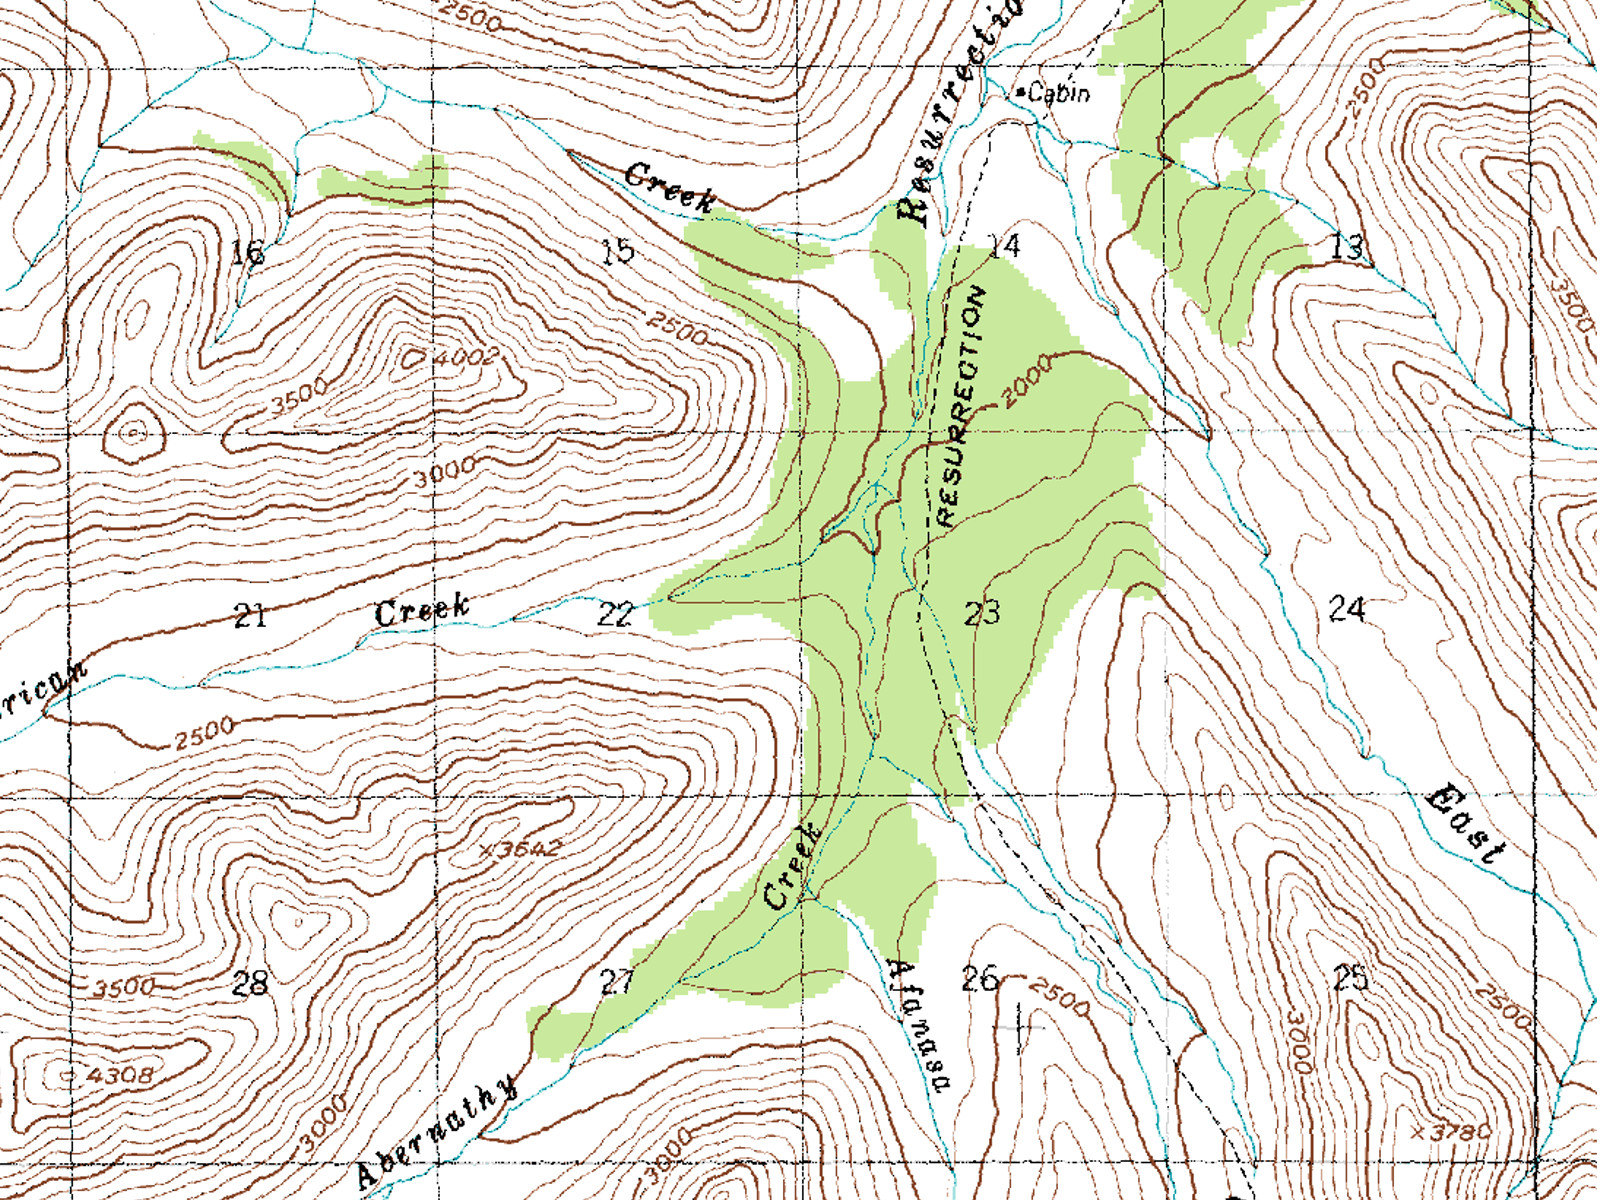
\includegraphics{topographicalmap.jpg}
\end{image}
In the map above, the contour curves are used to indicate elevation.\\
When several level curves of $f(x, y)$ are sketched in the same $xy$-plane, the figure is called a \textbf{contour map}.

\begin{example}[Example 3]
Describe the level curves of the function $z = f(x, y) = \sqrt{1-x^2 - y^2}$ and sketch a contour map consisting of at least 3 level curves.\\
The level curves have the form 
\[
\sqrt{1 - x^2 - y^2} = k
\]
for some constant, $k$. Note that if $k < 0$ then the graph is the empty set.\\
To recognize the curve in the $xy$-plane, square both sides and rearrange to get:
\[
x^2 + y^2 = 1- k^2 
\]
If $0 \leq k < 1$ this is a circle in the $xy$-plane with center at the origin and radius $\sqrt{1-k^2}$.\\
If $k = 1$, this is just the single point $(0, 0)$ and \\
if $k>1$ then the graph is the empty set.\\
In the figure below, the chosen values for $k$ are: $\,0, \frac23, \frac{9}{10}$ and  $1$.
The corresponding radii of the circles are: $\,1, \frac{\sqrt{5}}{3}, \frac{\sqrt{19}}{10}$ and $0$.

\begin{image}
\begin{tikzpicture}
\draw[thick,blue!70!white] (0, 0) circle (3.5);
\node[thick,blue!70!white] at (1.8, 3.4) {$k = 0$};
\draw[thick,red!70!white] (0, 0) circle (2.5);
\node[thick,red!70!white] at (1.34, 2.56) {$k = 2/3$};
\draw[thick,green!70!black] (0, 0) circle (1.5);
\node[thick,green!70!black] at (1, 1.6) {$k = 9/10$};
\filldraw (0,0) circle (0.07);
\node[thick] at (0.5, 0.2) {$k = 1$};
\draw[thick, <->] (-5, 0) -- (5,0) node[right]{$x$};
\draw[thick, <->] (0, -5) -- (0, 5) node[left]{$y$};
\node at (3.8, -0.3) {$1$};
\node at (-.3, 3.8) {$1$};
\node at (0, -5.5) {A contour map consisting of level curves of $f(x, y)= \sqrt{1 - x^2 - y^2}$};
\end{tikzpicture}
\end{image}

\end{example}

\begin{problem}(Problem 3a)
Describe the level curves of the function $f(x,y) = x - 2y$ and sketch a contour map consisting of at least 3 level curves.\\
\end{problem}

\begin{problem}(Problem 3b)
Describe the level curves of the function $f(x, y) = x^2 + 4y^2$ and sketch a contour map consisting of at least 3 level curves.\\
\end{problem}

\begin{problem}(Problem 3c)
Describe the level curves of the function $f(x, y) = \sqrt{x^2 + y^2}$ and sketch a contour map consisting of at least 3 level curves.\\
\end{problem}

\begin{problem}(Problem 3d)
Describe the level curves of the function $f(x,y) = y - e^x$ and sketch a contour map consisting of at least 3 level curves.\\
\end{problem}

\begin{remark}
The graph of a function of one variable, $y= f(x)$ can be thought of as the level curve of the function of two variables given by 
\[
g(x, y) = y-f(x)
\]
corresponding to $k = 0$.
\end{remark}

\section{Functions of Three Variables}
The volume of a rectangular solid is length $\times$ width $\times $ height, so we can think of the volume as a function of three variables:
\[
Volume = f(length, width, height)
\]
In general a function of three variables looks like $f(x, y, z)$.
The graph of such a function consists of the set of points in $\R^4$ of the form $(x, y, z, f(x, y, z)$.
Our humanity limits us to three dimensions or fewer, so we are unable to produce the graph of a function of three variables.
However, we can consider their level surfaces.

\begin{example}[Example 4]
Describe the level surfaces of the function $f(x, y, z) = x^2 + 4y^2 + 9 z^2$.\\
The level surfaces are produced by the equation
\[
f(x, y, z) = k
\]
for constants, $k$.\\
In this example, the corresponding equation is
\[
x^2 + 4y^2 + 9z^2 = k
\]
which is an ellipsoid for $k >0$, and just the single point $(0, 0, 0)$ for $k = 0$.
For $k<0$, the level surface is the empty set.
\end{example}

\begin{problem}(Problem 4)
Describe the level surfaces of the function $f(x, y, z) = x^2 + y^2 - z^2$.\\
\begin{hint}
Try $k = -1, 0, 1$
\end{hint}
\begin{hint}
Refer to the end of section 1.8 for the equations of hyperboloids and cones
\end{hint}
\end{problem}

\begin{remark}
The graph of a function of two variables, $z= f(x,y)$ can be thought of as the level surface of the function of three variables given by 
\[
g(x, y, z) = z-f(x,y)
\]
corresponding to $k = 0$.
\end{remark}

\end{document}
